\documentclass[uplatex]{suribt}
%\documentclass[oneside]{suribt}% 本文が * ページ以下のときに (掲示に注意)

\usepackage{hyperref}
\usepackage[most]{tcolorbox}
\tcbuselibrary{breakable, skins, theorems}
\usepackage{xcolor}
\usepackage{ulem}
\usepackage{amssymb,amsmath,amsfonts,amsthm}
\usepackage{mathtools}
\mathtoolsset{showonlyrefs=true}
\usepackage{booktabs,tabularx}
\usepackage{url}
\usepackage{graphicx}
\usepackage{autobreak}
\usepackage{lmodern}
\usepackage{braket,physics} 
\usepackage{bm}
\usepackage{latexsym}
\usepackage{comment}
\usepackage{pdfpages}
\usepackage{here}
\usepackage{multicol}
\setlength{\columnsep}{5mm}
\columnseprule=0.2mm
\usepackage{ascmac}
\usepackage{array}
\usepackage{enumitem}
\usepackage{physics}
\usepackage{lastpage}
\usepackage{cancel}
\usepackage{ulem} % ulemパッケージを追加
\usepackage{algorithm}
\usepackage{algpseudocode}
\usepackage{comment}


% ========= 数学の基本的な定義やショートカット =========
\newcommand{\R}{\mathbb{R}}
\newcommand{\Z}{\mathbb{Z}}
\newcommand{\N}{\mathbb{N}}
\newcommand{\C}{\mathbb{C}} 



\title{Reservoir Computer による\\外力付きカオス時系列予測と\\生体リズム研究への応用}
%\titlewidth{}% タイトル幅 (指定するときは単位つきで)
\author{久野 証}
\eauthor{Sho Kuno}% Copyright 表示で使われる
\studentid{03-210599}
\supervisor{郡 宏 教授}% 1 つ引数をとる (役職まで含めて書く)
%\supervisor{指導教員名 役職 \and 指導教員名 役職}% 複数教員の場合,\and でつなげる
\handin{2024}{2}% 提出月. 2 つ (年, 月) 引数をとる
%\keywords{キーワード1, キーワード2} % 概要の下に表示される


\begin{document}
\maketitle%%%%%%%%%%%%%%%%%%% タイトル %%%%

\frontmatter% ここから前文
\begin{abstract}%%%%%%%%%%%%% 概要 %%%%%%%%
 ここに概要を書く.
\end{abstract}

\tableofcontents%%%%%%%%%%%%% 目次 %%%%%%%%

\mainmatter% ここから本文 %%% 本文 %%%%%%%%

\chapter{はじめに}
\section{背景}
\section{本書の構成}
\clearpage
\chapter{前提知識}

\section{生体リズム研究}

\cite{koriAcceleratingRecoveryJet2017}

\cite{yamaguchiMiceGeneticallyDeficient2013a}

\section{力学系}
一般的な話.
\cite{strogatz2018nonlinear}とかを参考に一般論.


\subsection{Van Der Polモデル}

\begin{align}
    \frac{d^2 x}{d t^2}-\mu\left(1-x^2\right) \frac{d x}{d t}+x=0
\end{align}



\subsection{Rösslerモデル}
\clearpage
\section{Reservoir Computerの概要}

Reservoir ComputerはEcho State Network (ESN)の一つのモデルである.ESNはRecurrent Neural Network (RNN)の枠組みの一つで,学習の対象を出力層のみに限定することによって,従来のRNNと比較して学習コストを大幅に節約する.
ここでは,\cite{bolltExplainingSurprisingSuccess2021}に基づいて,Reservoir Computerの構造と原理について概説する.また,Reservoir Computerの理論的な背景についても,先行研究を交えながら触れる.

\textbf{構造.}
Reservoir Computerは,入力層(Input layer),レザバー層(Reservoir layer),出力層(Output/ Readout Layer)の三つの層から成る.


\begin{figure}[h]
    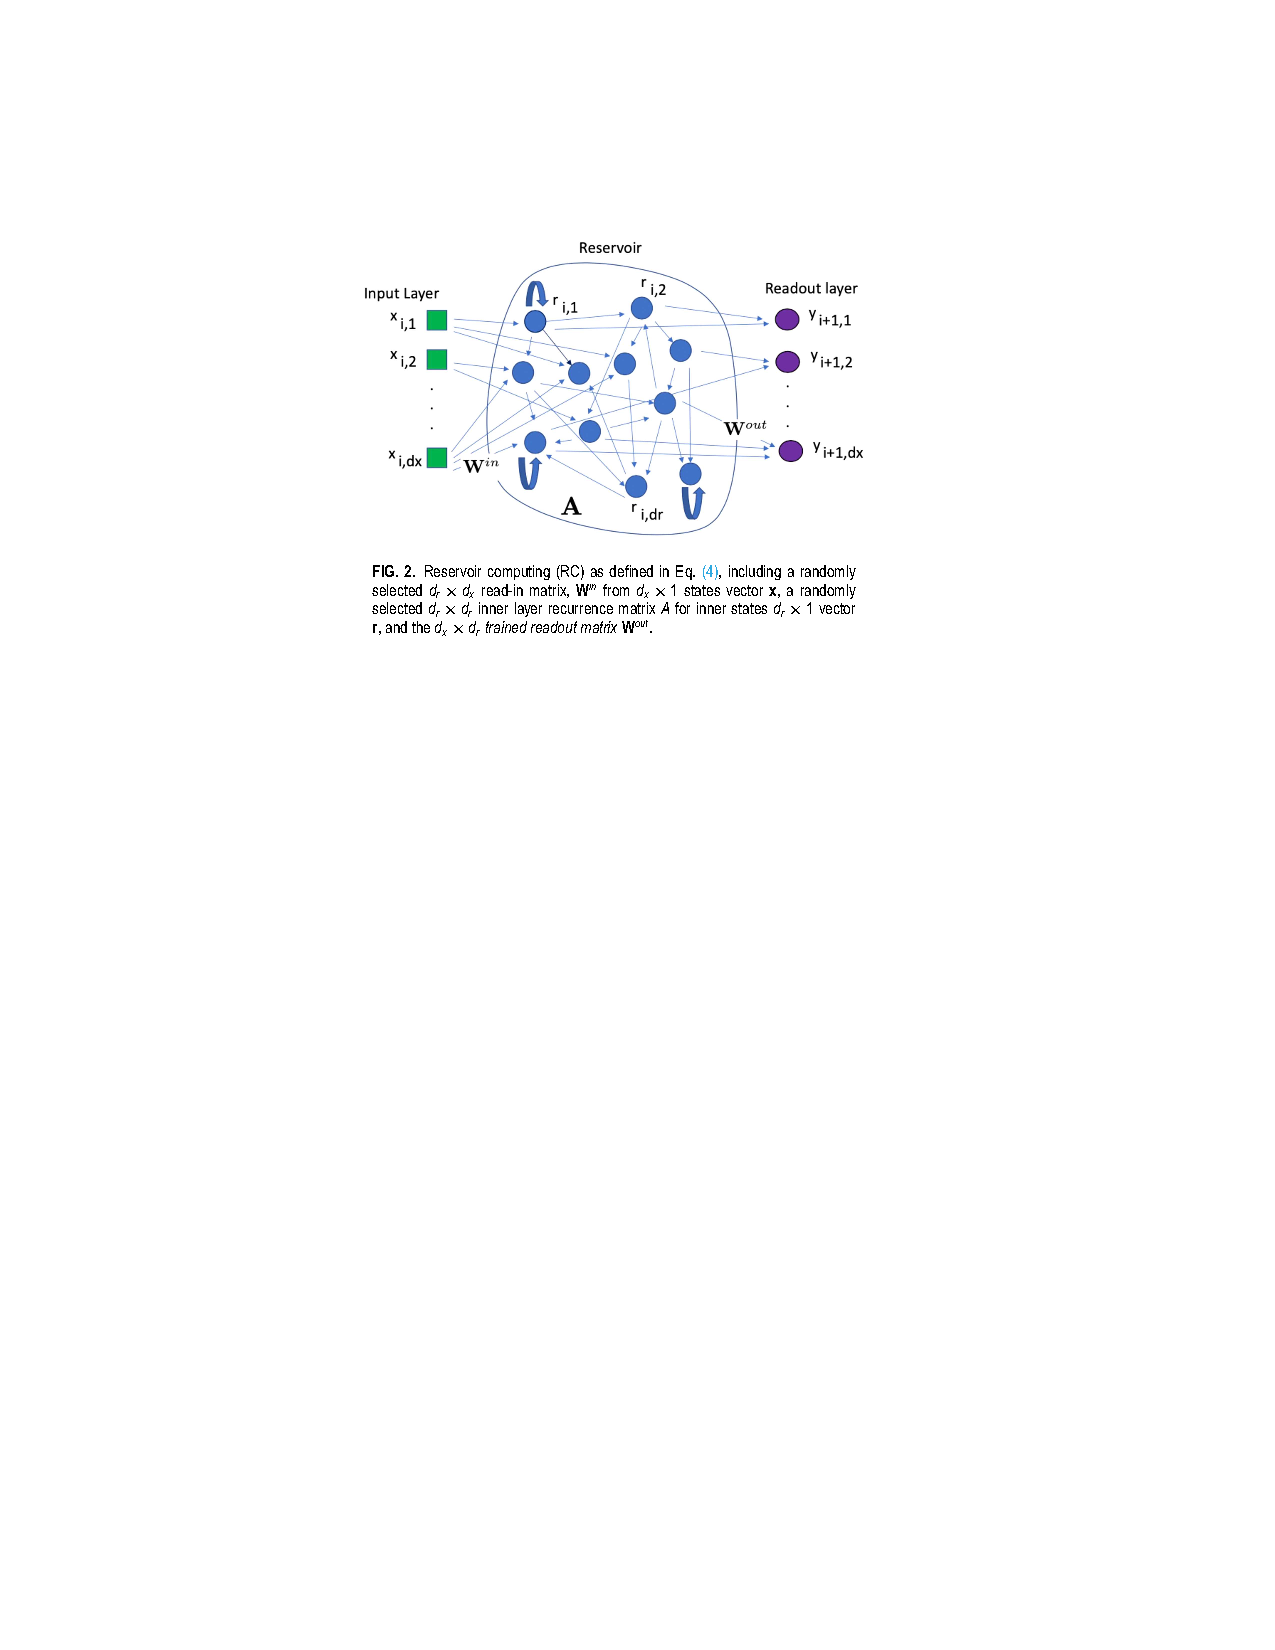
\includegraphics[width=\textwidth]{images/bollt.reservoir.pdf}
    \caption{}
\end{figure}  


\textbf{原理.}


\begin{comment}
    \begin{figure}[h]
    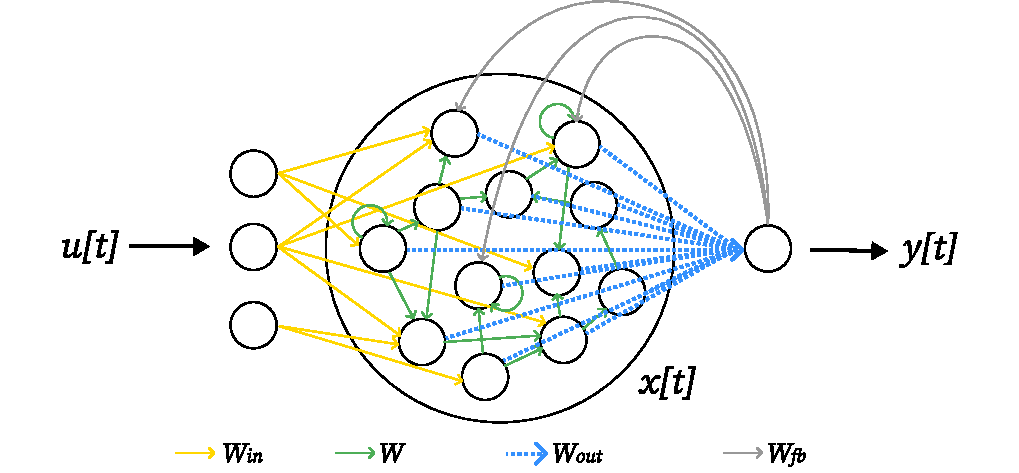
\includegraphics[width=\textwidth]{images/esn.pdf}
\end{figure}  
\begin{figure}[h]
    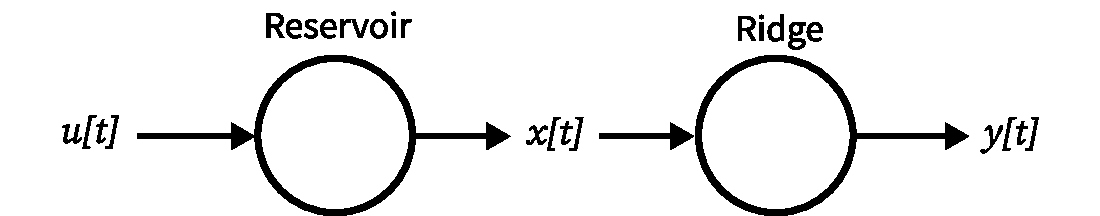
\includegraphics[width=\textwidth]{images/esn_nodes.pdf}
    \caption{}
\end{figure}  
\end{comment}


\textbf{理論的な背景.}
\cite{grigoryevaChaosCompactManifolds2021}
\cite{grigoryevaLearningStrangeAttractors2023}
\cite{berryLearningTheoryDynamical2023a}

Stochastic Inputsに対するuniversal approximationの話.
\cite{grigoryevaUniversalDiscretetimeReservoir2018}




\clearpage
\section{応用面での先行研究}


比較検討論文.二つくらいあってもいいかな.
\cite{zhangSurveyReservoirComputing2023}:Online learning/ force algorithm等に触れている.



\subsection{Y. Laiの研究内容}
本研究の直接的な先行研究として\cite{kongDigitalTwinsNonlinear2022}があるので,ここでその内容について紹介する.

\begin{figure}[h]
    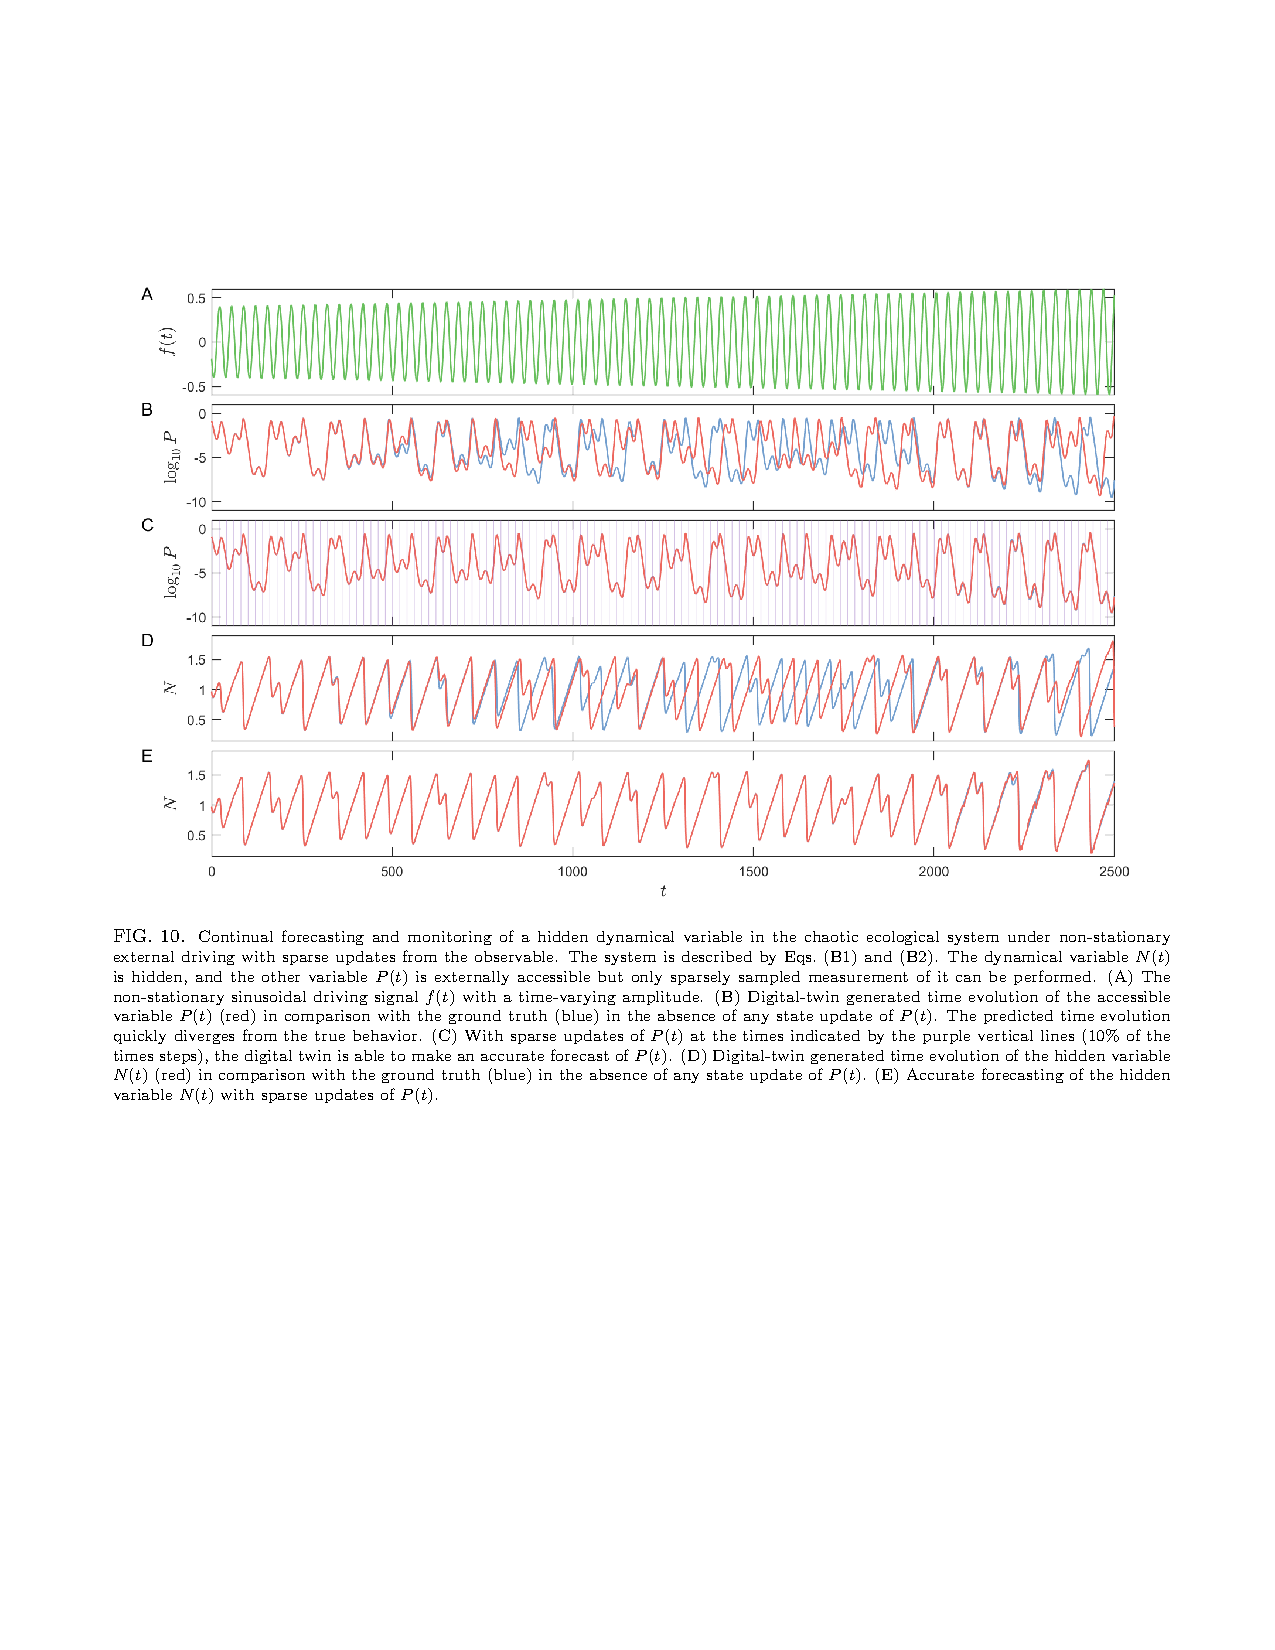
\includegraphics[width=\textwidth]{images/lai_result.pdf}
    \caption{}
\end{figure}  


\clearpage

\subsection{METHODS}
\begin{itemize}
    \item Digital twins: a recurrent RC neural network with a control
    mechanism, which requires two types of input signals:
    the observational time series for training and the con-trol signal $f(t)$ that remains in both the training and
    self-evolving phase. \begin{itemize}
        \item During the train-ing, the hidden recurrent layer is driven by both the in-
        put signal $u(t)$ and the control signal $f(t)$. 
    \end{itemize}
    \item Reservoir updating equations:
    \begin{align}
    \text{training phase: }& \mathbf{r}(t+\Delta t)=(1-\alpha) \mathbf{r}(t) + \alpha \tanh \left[\mathcal{W}_r \mathbf{r}(t)+\mathcal{W}_{\text {in }} \mathbf{u}(t)+\mathcal{W}_c f(t)\right] \\
    \text{self-evolving phase: } & \mathbf{r}(t+\Delta t)=(1-\alpha) \mathbf{r}(t) + \alpha \tanh \left[\mathcal{W}_r \mathbf{r}(t)+\mathcal{W}_{\text {in }} \mathcal{W}_{\text {out }} \mathbf{r}^{\prime}(t)+\mathcal{W}_c f(t)\right]
    \end{align}

    \item $\bold{“sense, learn, and mingle”}$: During
    the training, several trials of data are typically used un-der different driving signals so that the digital twin can
    the responses of the target sys-tem to gain the ability to extrapolate a response to a new driving signal that has never been encountered before. We input these trials of training data, i.e., a few pairs of $\mathbf{u}(t)$ and the associated $f(t)$, through the matrices $\mathcal{W}_{\text {in }}$ and $\mathcal{W}_c$ sequentially. 

    \item $\bold{validation/testing}$: the validation of the RC net-works are done with the same driving signals $f(t)$ as in
    the training data. We test driving signals $f(t)$ that are
    different from those generating the training data (e.g.,
    with different amplitude, frequency, or waveform).  

    \item $\bold{warming-up}$ During the warming-up process to initialize the RC networks prior to making the predictions, we feed randomly chosen short segments of the training time series to feed into the RC network.
    That is, no data from the target system under the testing
    driving signals $f(t)$ are required for making the predic-
    tions.
\end{itemize}


\clearpage


\subsection{RESULTS}


\chapter{議論}
\clearpage

\cite{RODRIGUES20161}

\backmatter% ここから後付
\chapter{謝辞}%%%%%%%%%%%%%%% 謝辞 %%%%%%%

%\begin{thebibliography}{}%%%% 参考文献 %%%
% \bibitem{}
%\end{thebibliography}
\bibliographystyle{unsrt}%           BibTeX を使う場合
\bibliography{reference.bib}% BibTeX を使う場合

\documentclass[../main]{subfiles}
\begin{document}
\chapter{鎖状ネットワークの同期に関する先行研究}
\label{chap:appendix}
\cite{XiaHuang:130506}の解析内容について述べる.\\
鎖状に無向グラフとして$N$個連なった位相振動子ネットワークのふるまいを以下で記述するとする.
\begin{align*}
    \dot{\theta}_1&=\omega_1\\
    \dot{\theta}_i&=\omega_i+\lambda\sin(\theta_{i-1}-\theta_i),\ i=2,3,\ldots,N
\end{align*}
ここで,$\theta_i,\omega_i$をそれぞれ端から$i$番目の振動子の位相と固有振動数とする.$\lambda>0$は振動子間の結合強度とする.
このモデルでは端の振動子$1$が固有振動数$\omega_1$をもつ駆動源となり,他の振動子は駆動源に近い方の隣接した振動子と相互作用する.\\

$\omega_1=2,\omega_2=1$とし,他の$\omega_i$をランダムに選択するとして固有振動数を配置し,結合強度を高めていく数値実験を行ったところ,4つのクラスタリングパターンが観測された.
\renewcommand{\labelenumi}{Case  \theenumi}
\begin{enumerate}
    \item \label{enu:case1} 隣接した駆動振動子と同期し局所クラスターが発生する.
    \item \label{enu:case2} 駆動源と同期する振動子が出現する.
    \item \label{enu:case3} 結合強度が小さい間は隣接した駆動振動子と同期し局所クラスターを構成した後,結合強度がある程度大きくなると局所クラスターが消滅する.
    \item \label{enu:case4} 隣接した駆動振動子が駆動源と同期した後,駆動される振動子自体も同期する.
\end{enumerate}
つまり,各振動子とクラスターを構成するのは,隣接した駆動振動子と,駆動源の2つの振動子のみである.
このパターンは,他の鎖状ネットワークでも普遍的であるため,これらのクラスタリングパターンの分岐を考える.

特に$N=3,\ \omega_1=2,\ \omega_2=1$とする.$\omega_3$を変化させたとき全部で4つの領域に分かれた.
\begin{itemize}
    \item $\omega_3\in[1,2]$のとき,結合強度の増加により隣接した駆動振動子と同期する.Case \ref{enu:case1}に相当する.
    \item $\omega_3\in(2,3]$のとき,結合強度の増加により駆動振動子と同期する.Case \ref{enu:case2}に相当する.
    \item $\omega_3\lesssim 1$のとき,結合強度が小さい間は隣接した駆動振動子と同期し局所クラスターを構成した後,結合強度がある程度大きくなると局所クラスターが消滅する.Case \ref{enu:case3}に相当する.
    \item $\omega_3$が$\omega_1,\omega_2$両方ともから離れた値のとき,隣接した駆動振動子が駆動源と同期した後,駆動される振動子自体も同期する.Case \ref{enu:case4}に相当する.
\end{itemize}
以上の分岐を調べるため,以下の方程式を考える.
\begin{align}
    \label{eq:3driving}
    \begin{split}
        \dot{\theta}_1&=\omega_1\\
        \dot{\theta}_2&=\omega_2+\lambda\sin(\theta_1-\theta_2)\\
        \dot{\theta}_3&=\omega_3+\lambda\sin(\theta_2-\theta_3)
    \end{split}
\end{align}
ここで,$\phi_{21}=\theta_2-\theta_1,\ \Delta\omega_{21}=\omega_2-\omega_1$とすると,
\begin{align}
    \label{eq:phasediff-21}
    \dot{\phi_{21}}=\Delta\omega_{21}-\lambda\sin\phi_{21}
\end{align}
となる.ここで,両辺の長時間平均$\langle\cdot\rangle$を考える.
$\lambda$が同期が起こらないくらい小さいとき,$\phi_{21}$の確率分布$\rho(\phi_{21},t)$は十分時間が経つと安定分布に収束する.
\begin{align*}
    \rho(\phi_{21},t)=\frac{\Delta\omega_{21}-\lambda\sin\phi_{21}}{C},\quad C:\mathrm{normalization\ constant}
\end{align*}
この確率分布に$\phi_{21}$が従うとして式\eqref{eq:phasediff-21}の$\sin\phi_{21}$を平均する.
すると,
\begin{align*}
    \langle\sin\phi_{21}\rangle=\frac{\Delta\omega_{21}-\sqrt{(\Delta\omega_{21})^2-\lambda^2}}{\lambda}
\end{align*}
よって,式\eqref{eq:3driving}より,$\theta_2$の実効振動数が得られる.
\begin{align*}
    \langle\dot{\theta}_2\rangle=\omega_1+\sqrt{(\Delta\omega_{21})^2-\lambda^2}
\end{align*}
この式より,$\lambda_c=\Delta\omega_{21}$として,$\lambda\geq\lambda_c$のとき$\langle\dot{\theta}_2\rangle=\omega_1$となり,振動子$1$と振動子$2$は同期する.
同様の手順で$\theta_3$の実効振動数が得られる.
\begin{align}
    \label{eq:effective-approx}
    \langle\dot{\theta}_3\rangle=\langle\dot{\theta}_2\rangle+\sqrt{(\Delta\omega_{32})^2-\lambda^2}
\end{align}
ただし,$\Delta\omega_{32}=\omega_3-\langle\dot{\theta}_2\rangle$である.\\
以上より,振動子の同期条件を求めることができる.
振動子$2$と振動子$3$の同期条件は
$\Delta\omega_{21}\geq 0$のとき,
\begin{align*}
    \begin{cases}
        -\lambda\leq\Delta\omega_{31}-\sqrt{(\Delta\omega_{32})^2-\lambda^2}\geq\lambda & (\lambda\leq|\Delta\omega_{21}|)\\
        -\lambda\leq\Delta\omega_{31}\geq\lambda & (\lambda>|\Delta\omega_{21}|)
    \end{cases}
\end{align*}
$\Delta\omega_{21}< 0$のとき,
\begin{align*}
    \begin{cases}
        -\lambda\leq\Delta\omega_{31}+\sqrt{(\Delta\omega_{32})^2-\lambda^2}\geq\lambda & (\lambda\leq|\Delta\omega_{21}|)\\
        -\lambda\leq\Delta\omega_{31}\geq\lambda & (\lambda>|\Delta\omega_{21}|)
    \end{cases}
\end{align*}
ここで,$\Delta\omega_{31}=\omega_3-\omega_1$である.
これらの同期条件から,$\omega_c=-\sqrt{2}|\Delta\omega_{21}|+\omega_1$という臨界振動数を境界とする領域$\omega_3\in(\omega_c,\omega_2)$でCase \ref{enu:case2}のような分離が起こることがわかる.\\
次に,振動子$1$と振動子$3$の同期条件を考える.
$\phi_{31}=\theta_3-\theta_1$とすると,
\begin{align*}
    \dot{\phi}_{31}=\Delta\omega_{31}-\lambda\sin(\phi_{31}-\phi_{21})
\end{align*}
となるから同期の必要条件は,$|\Delta\omega_{31}|\leq \lambda$となる.
また,$\langle\dot{\theta}_3\rangle=\omega_1$の状況を考えると,式\eqref{eq:effective-approx}から,同期の十分条件が求まる.
\begin{align*}
    \omega_3\leq\omega_1+|\Delta\omega_{21}|-\sqrt{(\Delta\omega_{21})^2-\lambda^2}
\end{align*}
以上の解析から$\omega_3,\lambda$と同期クラスタの関係が図\ref{fig:appendix-bifurcation}として示される.
\begin{figure}[t]
\centering
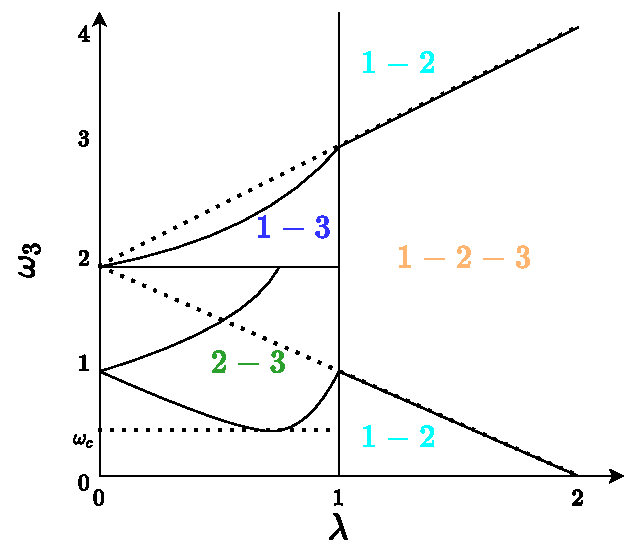
\includegraphics[width=70mm]{./images/appendix-bifurcation.pdf}
\centering
\caption{$\omega_1=2,\ \omega_2=1$のときの固有振動数$\omega_3$と結合強度$\lambda$に対する相図.
あるパラメータ領域で同期クラスタが発生する場合,その振動子の組を各領域に示している.また,同期クラスタが異なるパラメータ領域の境界を実線で示している.}
\label{fig:appendix-bifurcation}
\end{figure}
また,式\eqref{eq:effective-approx}を再帰的に利用することで$N>3$の場合でも同様の解析が可能となる.
\end{document}
\end{document}